\section{Genuine and Imposter Distributions}
\label{sec:experiment:distribution}

Figure ~\ref{fig:experiment:11a} through ~\ref{fig:experiment:11o} show the genuine and imposter distributions when the 15-dimensional features are applied to the 4000 training database when only the $i$th dimension is used to calculate the Euclidian distance. Figure ~\ref{fig:experiment:11p} shows the result when all 15 dimensions are used together.

\begin{figure}[htb]
  \begin{center}
    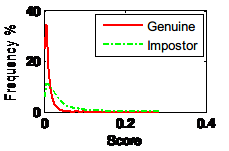
\includegraphics[scale=1]{ch-experiment/figures/11a}
    \caption{Genuine and imposter distributions by matching the 1st dimension}
    \label{fig:experiment:11a}
  \end{center}
\end{figure}

\begin{figure}[htb]
  \begin{center}
    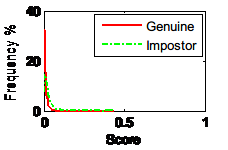
\includegraphics[scale=1]{ch-experiment/figures/11b}
    \caption{Genuine and imposter distributions by matching the 2nd dimension}
    \label{fig:experiment:11b}
  \end{center}
\end{figure}

\begin{figure}[htb]
  \begin{center}
    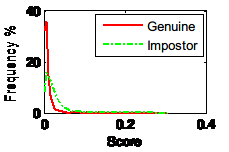
\includegraphics[scale=1]{ch-experiment/figures/11c}
    \caption{Genuine and imposter distributions by matching the 3rd dimension}
    \label{fig:experiment:11c}
  \end{center}
\end{figure}

\begin{figure}[htb]
  \begin{center}
    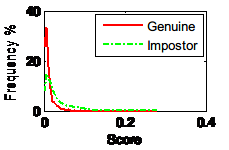
\includegraphics[scale=1]{ch-experiment/figures/11d}
    \caption{Genuine and imposter distributions by matching the 4th dimension}
    \label{fig:experiment:11d}
  \end{center}
\end{figure}

\begin{figure}[htb]
  \begin{center}
    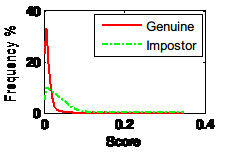
\includegraphics[scale=1]{ch-experiment/figures/11e}
    \caption{Genuine and imposter distributions by matching the 5th dimension}
    \label{fig:experiment:11e}
  \end{center}
\end{figure}

\begin{figure}[htb]
  \begin{center}
    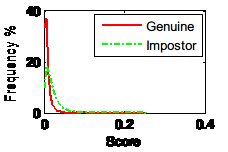
\includegraphics[scale=1]{ch-experiment/figures/11f}
    \caption{Genuine and imposter distributions by matching the 6th dimension}
    \label{fig:experiment:11f}
  \end{center}
\end{figure}

\begin{figure}[htb]
  \begin{center}
    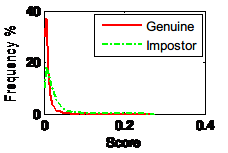
\includegraphics[scale=1]{ch-experiment/figures/11g}
    \caption{Genuine and imposter distributions by matching the 7th dimension}
    \label{fig:experiment:11g}
  \end{center}
\end{figure}

\begin{figure}[htb]
  \begin{center}
    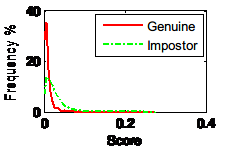
\includegraphics[scale=1]{ch-experiment/figures/11h}
    \caption{Genuine and imposter distributions by matching the 8th dimension}
    \label{fig:experiment:11h}
  \end{center}
\end{figure}

\begin{figure}[htb]
  \begin{center}
    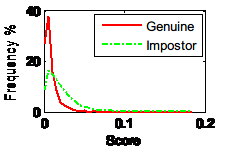
\includegraphics[scale=1]{ch-experiment/figures/11i}
    \caption{Genuine and imposter distributions by matching the 9th dimension}
    \label{fig:experiment:11i}
  \end{center}
\end{figure}

\begin{figure}[htb]
  \begin{center}
    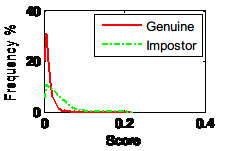
\includegraphics[scale=1]{ch-experiment/figures/11j}
    \caption{Genuine and imposter distributions by matching the 10th dimension}
    \label{fig:experiment:11j}
  \end{center}
\end{figure}

\begin{figure}[htb]
  \begin{center}
    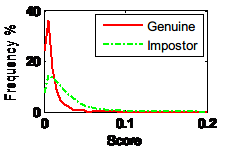
\includegraphics[scale=1]{ch-experiment/figures/11k}
    \caption{Genuine and imposter distributions by matching the 11th dimension}
    \label{fig:experiment:11k}
  \end{center}
\end{figure}

\begin{figure}[htb]
  \begin{center}
    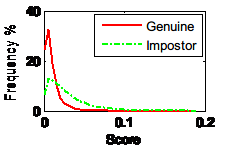
\includegraphics[scale=1]{ch-experiment/figures/11l}
    \caption{Genuine and imposter distributions by matching the 12th dimension}
    \label{fig:experiment:11l}
  \end{center}
\end{figure}

\begin{figure}[htb]
  \begin{center}
    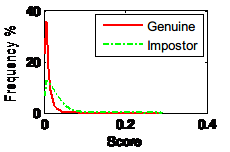
\includegraphics[scale=1]{ch-experiment/figures/11m}
    \caption{Genuine and imposter distributions by matching the 13th dimension}
    \label{fig:experiment:11m}
  \end{center}
\end{figure}

\begin{figure}[htb]
  \begin{center}
    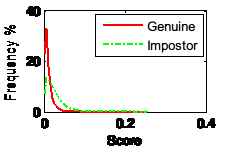
\includegraphics[scale=1]{ch-experiment/figures/11n}
    \caption{Genuine and imposter distributions by matching the 14th dimension}
    \label{fig:experiment:11n}
  \end{center}
\end{figure}

\begin{figure}[htb]
  \begin{center}
    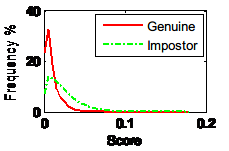
\includegraphics[scale=1]{ch-experiment/figures/11o}
    \caption{Genuine and imposter distributions by matching the 15th dimension}
    \label{fig:experiment:11o}
  \end{center}
\end{figure}

\begin{figure}[htb]
  \begin{center}
    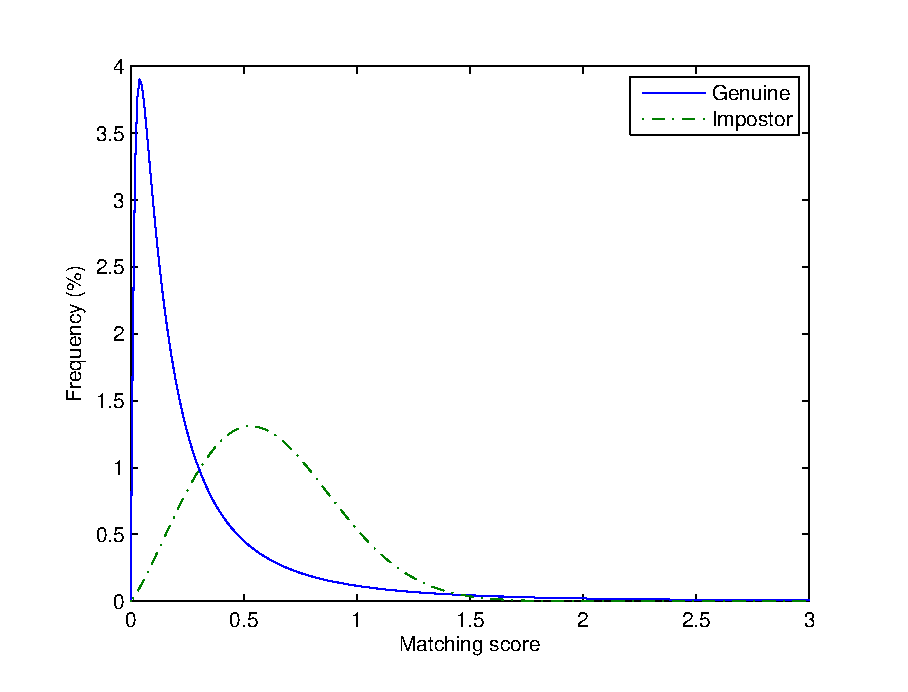
\includegraphics[scale=1]{ch-experiment/figures/11p}
    \caption{Genuine and imposter distributions by matching all the 15 dimensions}
    \label{fig:experiment:11p}
  \end{center}
\end{figure}

